\documentclass{book}
\usepackage{commeunjeustyle}
\begin{document}


\chapter*{Application linéaire}


\begin{Texte}
Comme souvent en mathématiques, ce sont plus les transformations qui sont intéressantes et pertinentes que les objets eux-mêmes.\\
Une application linéaire est un cas particulier de transformation.  Dans le langage courant, un phénomène est dit linéaire si les
effets sont proportionnels aux causes. \\
Plus précisément, un phénomène peut être décrit par une transformation$x \mapsto f (x)$, où $x$ représente la ou les causes (par exemple une différence de
potentiel) et $f(x)$ un effet auquel on s'intéresse (par exemple l'intensité
d'un courant électrique). On dit que le phénomène est linéaire quand  l'effet est proportionnel à la cause (exemple : l'intensité de courant est
proportionnel à la différence de potentiel, en d'autres termes, si on double
la différence de potentiel, on double l'intensité du courant résultant, si on somme de deux différence de potentiel, on somme l'intensité du courant résultant).
Beaucoup de phénomènes en sciences ne sont pas linéaires. Dans de tels
cas, de "petites causes" peuvent avoir de "grands effets".\\
D'un point de vue mathématiques, une
transformation préservant la structure d'espace vectoriel est une application linéaire.  Les matrices sont des tableaux de nombres qui servent à interpréter en termes calculatoires et donc opérationnels les applications linéaires dont les espaces vectoriels sont de dimensions finies.\\ 
\begin{Exemple}[Taille d'un père et d'un fils]
La somme des tailles d'un fils et du père est de 2,5 mètres. La différence de tailles  est de 0.5 mètres.
Quel est la taille du fils ? \\
Soit la variable $x$ représentant la taille du fils et la variable $y$ représentant la taille du père.\\
Le couple $(x,y)$ vérifie le système suivant  :
$$(S)\quad \begin{cases}
x+y&=2,5\\
-x+y&=0,5
\end{cases}
$$
L'idée est de considérer les membres de gauche des équations comme l'image d'une fonction :
\begin{center}
$
\begin{cases}
{\color{red}x}+{\color{green}y}&={\color{blue}2,5}\\
{\color{red}-x}+{\color{green}y}&={\color{blue}0,5}
\end{cases}
\Leftrightarrow\quad \begin{pmatrix}
 {\color{red}x} +{\color{green}y}   \\
 {\color{red}-x} +{\color{green}y}   \\
\end{pmatrix} =\begin{pmatrix}
 {\color{blue}2,5}   \\
 {\color{blue}0,5}  \\
\end{pmatrix}
\Leftrightarrow\quad
u(\begin{pmatrix}
 \color{red}x     \\ {\color{green}y}   \\
\end{pmatrix})
	 = \begin{pmatrix}
 {\color{blue}2,5}   \\
 {\color{blue}0,5}  \\
\end{pmatrix}$\\
\begin{tikzpicture}[general,scale=1]
\draw [->, epais] (0,0)node[left]{avec $\quad \begin{pmatrix}
 {\color{red}x}    \\
{\color{green}y}   \\
\end{pmatrix}$} -- (1,0);
\draw [-, epais] (1,-1)--(2.5,-1)--(2.5,1)--(1,1)--(1,-1);
\draw(1.75,0) node{$u$};
\draw [->, epais] (2.5,0) -- (3.5,0)node[right]{$\begin{pmatrix}
 {\color{red}x} + {\color{green}y}    \\
 {\color{red}-x}+  {\color{green}y}   \\
\end{pmatrix}$};
\end{tikzpicture} 
\end{center}
Les solutions du système sont l'ensemble des antécédents $\begin{pmatrix}
 {\color{blue}2,5}   \\
 {\color{blue}0,5}  \\
\end{pmatrix}$ de la fonction à deux variables $\Fonction{u}{\R^2}{\R^2}{\begin{pmatrix}
  {\color{red}x}    \\
 {\color{green}y}   \\
\end{pmatrix}}{\begin{pmatrix}
  {\color{red}x} +{\color{green}y}   \\
  {\color{red}-x} +{\color{green}y}   \\
\end{pmatrix}}$.\\
L'étude générale des fonctions à plusieurs variables est compliquée et est fait dans un cours d'analyse.  
Cependant, comme la fonction $u$ est linéaire :
 $$u(\begin{pmatrix}
 {x}    \\
{y}   \\
\end{pmatrix}+\begin{pmatrix}
 {x'}    \\
{y'}   \\
\end{pmatrix})=u(\begin{pmatrix}
 {x}    \\
{y}   \\
\end{pmatrix})+u(\begin{pmatrix}
 {x'}    \\
{y'}   \\
\end{pmatrix}) \quad\text{ et }\quad u(\lambda \begin{pmatrix}
 {x}    \\
{y}   \\
\end{pmatrix})=\lambda u(\begin{pmatrix}
 {x}    \\
{y}   \\
\end{pmatrix})$$
on aura des outils pour démontrer que $u$ est un isomorphisme. Ainsi il existe une unique vecteur antécédent au vecteur $\begin{pmatrix}
 {\color{blue}2,5}   \\
 {\color{blue}0,5}  \\
\end{pmatrix}$. Le système admet une unique solution.
\end{Exemple}
Notations :
\begin{itemize}
\item $\K $ désigne le corps $\R $ ou $\C $
\item $E$ et $F$ deux $\K$-espaces vectoriels
\end{itemize}
\end{Texte}


\section{Applications linéaires}

\subsection{Définition}



\begin{Definition}[Application linéaire]
Soit $E$ et $F$ deux $\K $-espaces vectoriels.\\
Une application $u:E\to F$ est dite \defi{linéaire}, si  elle préserve la structure d'espace vectoriel, c'est à dire si :
\begin{itemize}
\item
  \defi{additivité} : $\forall   \Vect{x},\Vect{y}\in  E:\quad u(\Vect{x}+\Vect{y}) = u(\Vect{x}) + u(\Vect{y})$;
\item
  \defi{homogénéité} : $\forall   \lambda \in  \K,\forall   \Vect{x}\in  E:\quad u(\lambda \Vect{x}) = \lambda u(\Vect{x})$.
\end{itemize}
\end{Definition}
\begin{Exemple} 
\begin{itemize}
\item homothétie vectorielle de rapport $\lambda$ : $\Fonction{\Phi _0}{E}{E}{\Vect{x}}{\lambda\vec{x}}$ 
\item Équation d'un plan : $\Fonction{\Phi _1}{\mathbb {R}^3 }{\mathbb {R}}{(x,y,z)}{x+y+3z}$,
\item Intégration :$\Fonction{\Phi _2}{\mathcal{C}([0,1]),  \mathbb {R} }{\mathbb {R}}{f}{\int_0^1 f(x)dx}$,
\item Dérivé de polynôme de degré au plus $n$ : $\Fonction{\Phi _3}{\mathbb {R}_n[X] }{\mathbb {R}_n[X]}{P}{P'}$,
\end{itemize}
\end{Exemple}


\begin{DefinitionProposition}[Modélisation d'une situation de proportionnalité]
Deux quantités $x$ et $y$ réelles sont \defi{proportionnelles} quand, en multipliant par une constante $a$, appelé \defi{coefficient de proportionnalité},  une quantité, on obtient l'autre. La représentation fonctionnelle  de cette relation est définie par  $$u:x\to ax =$$ où $y=u(x)$.\\
$u$ est une fonction linéaire de $\R$ dans $\R$.
\end{DefinitionProposition}
\begin{Demonstration}
\begin{itemize}
\item additivité : Soit $x_1,x_2\in \R$.\\
$$u(  x_1+x_2)=a(  x_1+x_2)=ax_1+ax_2=u(x_1)+u(x_2)$$
\item homogénéité : Soit $\lambda\in\R, x\in \R$.\\
$$u(\lambda  x)=a( \lambda x)=\lambda a x=\lambda u(x).$$
\end{itemize} 
\end{Demonstration}

\begin{Exemple}[Essence]
Le prix à la pompe est proportionnel du volume d'essence mis dans le réservoir.
\end{Exemple}
\begin{Exemple}[Différentielle]
Soit $f:\R \rightarrow \R $ une fonction dérivable en $a$. On a  
$$\overbrace{f(a+h)-f(a)}^{\text{accroissement de la fonction}}=\overbrace{\mathrm {d}f_a(h)}^{\text{terme linéaire}}+\overbrace{h.\epsilon(h)}^{\text{petit terme correctif}}$$ où l'application $\mathrm {d}f_a$, appelé différentielle de $f$ en $a$, est linéaire : $\mathrm {d}f_a(h)=f'(a).h$ avec $f'(a)$ le coefficient de proportionnalité.
\end{Exemple}

\begin{DefinitionProposition}[Modélisation d'une situation de linéarité]
Deux quantités $X=\begin{pmatrix}
x_1\\\vdots\\x_p
\end{pmatrix}$ et $Y=\begin{pmatrix}
y_1\\\vdots\\y_n
\end{pmatrix}$ sont en relation \defi{linéaires} quand chaque coefficient de $Y$ s'exprime comme combinaison linéaire des coefficients de $X$, c'est à dire :
$$
\begin{cases}
y_1=&a_{11}x_1+\dots+a_{1p}x_p\\
\vdots&\vdots\\
y_n=&a_{n1}x_1+\dots+a_{np}x_p
\end{cases}
$$
La représentation matricielle de cette relation est définie par :$$\Fonction{u}{\R^p}{\R^n}{X}{AX}.$$ avec la matrice $A=\begin{pmatrix}
a_{11}&\dots&a_{1p}\\\vdots&\vdots\\a_{n1}&\dots&a_{np}
\end{pmatrix}$.\\
  $u$ est une fonction linéaire de $\R^p$ dans $\R^n$.
\end{DefinitionProposition}
\begin{Demonstration}
\begin{itemize}
\item additivité : Soit $X_1,X_2\in \R^p$.\\
$$u(  X_1+X_2)=A(  X_1+X_2)=AX_1+AX_2=u(X_1)+u(X_2)$$
\item homogénéité : Soit $\lambda\in\R, X\in \R^p$.\\
$$u(\lambda  X)=A( \lambda X)=\lambda A X=\lambda u(X).$$
\end{itemize} 
\end{Demonstration}
\begin{Exemple}[Transformation linéaire du plan]
La rotations, l'homothétie, la transvection et la   symétrie axiale sont des transformations linéaires du plan. 
\begin{center}
\begin{Figure}
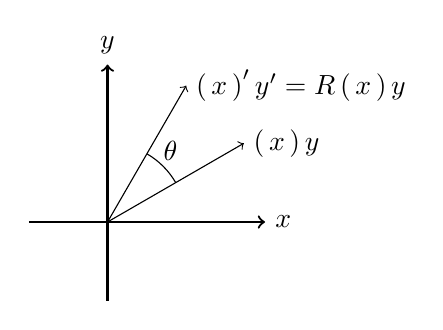
\begin{tikzpicture}
\draw[thick,->] (-1,0) -- (2,0)node[anchor=west] {$x$};
\draw[thick,->] (0,-1) -- (0,2)node[anchor=south] {$y$};
\draw (0.866,0.5) arc (30:60:1) ;
\draw[->] (0,0)--(1.732,1) node[right] {$\begin{pmatrix} x \\ y \end{pmatrix}$};
\draw[->] (0,0)-- (1,1.732) node[right] {$\begin{pmatrix} x '\\ y' \end{pmatrix}=R\begin{pmatrix} x \\ y \end{pmatrix}$};
\node at (0.8,0.9){$\theta$};
\end{tikzpicture}

\begin{Titre}
Pour une rotation anti-horaire autour de l'origine, on a  $x '= x \cos \theta -y \sin \theta$ et $y ' = x \sin \theta + y \cos \theta$ et sous la forme matricielle : $\begin{pmatrix} x '\\ y' \end{pmatrix} = R \begin{pmatrix} x \\ y \end{pmatrix}$ avec $R=\begin{pmatrix}
\cos \theta & -\sin \theta\\
\sin \theta & \cos \theta\\
\end{pmatrix}$
\end{Titre}
\end{Figure}
\end{center}
\end{Exemple}









\begin{Definition}[Endomorphisme]
\begin{itemize}
\item
  Une application linéaire dont l'espace de départ est le même que celui d'arrivée est un \defi{endomorphisme}.
\item
  Un \defi{isomorphisme} est une application linéaire bijective.
\item
  Un \defi{automorphisme} est un endomorphisme bijectif.
\end{itemize}
\end{Definition}
\begin{Exemple}
$\Phi _3$ et $R_\theta$ sont des endomorphismes. Comme $R_\theta$ est bijectif, $R_\theta$ est un automorphisme. 
\end{Exemple}
\begin{Texte}
Un isomorphisme permet de transporter les propriétés vectoriels entre les deux espaces vectoriels, par exemple la dimension.  Toute propriété ``vectorielle'' vraie pour un espace vectoriel donné sera vraie pour un espace vectoriel qui lui est isomorphe. \\ 
Par exemple on identifie fréquemment les $p$-uplets avec les matrices colonnes 
car l'application
\[ \Fonction{\Phi }{\K ^p}{\M{p}{1}{\K}}{(\lambda_1,\dots,\lambda_p)}{\begin{pmatrix}\lambda_1\\\vdots\\\lambda_p\end{pmatrix}} \]
est un isomorphisme.\\
Ainsi, on notera $X=\begin{pmatrix}x_1\\x_2\\\end{pmatrix}\overbrace{=}^{\text{identification}}(x_1,x_2)=\Vect{x}.$
\end{Texte}










\begin{DefinitionProposition}[Espace vectoriel des application linéaires et endomorphismes]
Soit $E$ et $F$ deux $\K $-espaces vectoriels.
L'ensemble des applications linéaires de $E$ dans $F$ est noté \defi{$\mathcal{L}(E,F)$} ;
il s'agit d'un sous espace vectoriel de l'espace des fonctions de $E$ dans $F$ muni des lois usuelles.\\
L'espace vectoriel des endomorphismes de $E$ se note \defi{$\LE$}$= \mathcal{L}(E,E)$.
\end{DefinitionProposition}
\begin{Demonstration}
Tous les axiomes se vérifient aisément.  
\end{Demonstration}
\begin{Definition}[composition d'application linéaire]
La \defi{loi de composition interne $\circ$} est définie comme une composition de fonctions, c'est à dire si $u\in\mathcal{L}(E,F)$ et $v\in\mathcal{L}(F,G) $,
 alors  $\forall \Vect{x} \in E : (v\circ u)(\Vect{x})=v(u(\Vect{x}))$.\\
On a $v\circ u\in \mathcal{L}(E,G).$
 \end{Definition}
\begin{Exemple}
L'application $P\mapsto XP'(X^2)$ est un endomorphisme de $\K[X]$. Les applications $P\mapsto P'$, $P\mapsto P(X^2)$ et $P\mapsto XP$ sont linéaire, donc par composition  $P\mapsto XP'(X^2)$ l'est aussi.    
\end{Exemple} 
\begin{Definition}[Structure d'algèbre des endomorphismes]
L'\defi{élément neutre} de la composition dans $\LE$ est l'application identité, $Id_{E}:x\mapsto x$. L'endomorphisme $u^{-1}$ est appelé l' \defi{endomorphisme inverse} de $u$ si $ u^{-1}×u=u×u^{-1}=Id_{E}$. Dans ce cas, l'endomorphisme $u$ est dite \defi{inversible}.  $\LE$ possède une structure d'algèbre non commutative. L'espace vectoriel des automorphismes de $E$ se note $ \GLE$.   $(\GLE,\circ)$ est un groupe, appelé \defi{groupe linéaire}.
\end{Definition}

\subsection{Propriétés}
\begin{Proposition}[0 image de 0]
Soit $u:E\to F$ une application linéaire.\\
Alors $u(\Vect{0_E})=\Vect{0_F}$
\end{Proposition}
\begin{Demonstration}
$u(\Vect{0_E})\overbrace{=}^{\text{Elt neutre}}u(\Vect{0_E}+\Vect{0_E})\overbrace{=}^{\text{linéarité}}=u(\Vect{0_E})+u(\Vect{0_E})$. En ajoutant  $-u(\Vect{0_E})$ aux deux membres de l'égalité, on obtient $u(\Vect{0_E})=\Vect{0_F}$.
\end{Demonstration}
\begin{Exemple} 
L'application $f(x,y)\mapsto (x+y,1)$ n'est pas linéaire car $f(0,0)=(0,1).$ d'après la contraposée de la proposition précédente. 
\end{Exemple}
\begin{Proposition}[Caractérisation de la linéarité]
$u:E\to F$ est linéaire si et seulement si
$$\forall   \lambda  \in  \K , \forall   \Vect{x},\Vect{y}\in  E:\quad u(\lambda \Vect{x} +  \Vect{y}) = \lambda u(\Vect{x}) +  u(\Vect{y}).$$
\end{Proposition}
\begin{Demonstration}
\begin{itemize}
\item $(\Longrightarrow)$  soit $\lambda  \in  \K ,    \Vect{x},\Vect{y}\in E$
$$u(\lambda \Vect{x} +  \Vect{y})\overbrace{=}^{\text{additivité}}u(\lambda \Vect{x}) +  u(\Vect{y})\overbrace{=}^{\text{homogénéité}}\lambda u( \Vect{x}) +  u(\Vect{y}).$$
\item $(\Longleftarrow)$ 
\begin{itemize}
\item additivité : soit  $\Vect{x},\Vect{y}\in  E$. On a :
$$u(\Vect{x}+\Vect{y})=u(1\Vect{x}+\Vect{y})=1u(\Vect{x})+u(\Vect{y})=u(\Vect{x})+u(\Vect{y})$$
\item homogénéité : soit  $\Vect{x}\in  E,\lambda\in\K$. On a :
$$u(\lambda\Vect{x})=u(\lambda\Vect{x}+\Vect{0})=\lambda u(\Vect{x})+u(\Vect{0})\overbrace{=}^{u \text{ additive}}\lambda u(\Vect{x})+\Vect{0}=\lambda u(\Vect{x})$$
\end{itemize}
\end{itemize}
\end{Demonstration}

 \begin{Proposition}[Propriétés algébriques]
\begin{itemize}
\item
  \propri{Associativité} : $$(u \circ v) \circ w =u \circ( v \circ w).$$
\item
  \propri{Bilinéarité} : 
  $$ (\lambda u + \mu v) \circ w = \lambda u\circ w + \mu v\circ w\text{ et }u\circ (\lambda v+ \mu w) =\lambda u\circ v + \mu u\circ w.$$
\end{itemize}
\end{Proposition}
\begin{Demonstration}
La composition des fonctions est associative donc en particulier les fonctions linéaires aussi.\\
Les fonctions sont linéaires à gauche. En revanche, il faut l'hypothèse de linéarité pour la linéarité à droite. En effet, soit $\Vect{x}\in E$. On a :
$$u\circ (\lambda v+ \mu w)(\Vect{x})=u(\lambda v(\Vect{x})+ \mu w(\Vect{x}))\overbrace{=}^{\text{linéarité de }u}=\lambda u(v(\Vect{x})) + \mu u(w(\Vect{x})).$$
\end{Demonstration}

\begin{Remarque} On omet le plus souvent le symbole  $\circ$ : $v\circ u =v u$.
\end{Remarque}
%TODO METTRE UN EXEMPLE
\subsection{Caractérisation par l'image d'une base}
\begin{Theoreme}[Caractérisation par l'image d'une base]
Pour connaître/définir une application linéaire complètement, il suffit de connaître/définir les  images d'une base de l'espace vectoriel de départ. 
\end{Theoreme}
\begin{Remarque}
Pour déterminer une application quelconque, on n'a pas d'autre choix que de déterminer les images de chaque point $x\mapsto f(x)$. En revanche,   une application linéaire est complètement déterminer par l'image d'une base. Par exemple, soit $u:(x,y)\mapsto u(x,y)$ une application linéaire avec les images de base canonique : $u(1,0)=(1,1)$ et $u(0,1)=(1,-1)$. On a 
$$u(x,y)=u(x(1,0)+y(0,1))\overbrace{=}^{\text{linéarité}}x.u(1,0)+ y.u(0,1)=x.(1,1)+ y.u(1,-1)=(x+y,x-y).$$    
\end{Remarque}
\begin{Demonstration}
Soit $\mathcal{B}=(\Vect{e_1},\dots,\Vect{e_p})$ une base de $E$.\\
Comme $u$ est linéaire, on a :
\begin{align}
u(\Vect{x})&=u(\lambda_1.\Vect{e_1}+\dots +\lambda_p.\Vect{e_p})\\
u(\Vect{x})&=\lambda_1.u(\Vect{e_1})+\dots +\lambda_p.u(\Vect{e_p})
\end{align}
Cela implique que l'application linéaire $u$ est entièrement déterminée par les vecteurs $(u(\Vect{e_1}),\dots,u(\Vect{e_p}))$.
\end{Demonstration}

\begin{Theoreme}[Géométrisation d'un espace vectoriel de dimension finie]%label=applications_lineaires__geometrisation
Tout $\K$-espace vectoriel de dimension $n$ est isomorphe à $\K^n$.   
\end{Theoreme}
\begin{Demonstration}
Soit $E$ un $\K$-espace vectoriel de de dimension $n$. Il existe une base $\mathcal{B}=\{\Vect{e_1},\dots,\Vect{e_n}\}$ de $E$.\\
Soit  $\mathcal{B}=\{\Vect{f_1},\dots,\Vect{f_n}\}$ la base canonique de $\K^n$.\\
L'application linéaire $\phi$ de $E$ dans  $\K^n$ définie par $\phi(\Vect{e_i})=\Vect{f_i}$ est un isomorphisme. 
\end{Demonstration}
\begin{Exemple}[Géométrisation de ${\K_2[X]}$]
L'application linéaire $\Fonction{\phi}{\R_3}{\R_2[X]}{(a,b,c)}{a + bX + cX^2}$ est un isomorphisme qui "géométrise" $\R _2[X]$.\\
La coplanarité des vecteurs $(0, 1, 0)$, $(0, 0, 1)$ et $(0, 1, \frac 1 2)$   se traduit dans $\R_2[X]$ par celle des vecteurs $X$, $X^2$ et $X +\frac 1 2  X^2$.
\begin{center}
\begin{Figure}
\begin{tikzpicture}
\draw[color=colordef,->] (0,0) -- (-0.7,-0.7)node[left] {$(1,0,0)$};
\draw[color=colordef,->] (0,0) -- (0.9,-0.2)node[right] {$(0,1,0)$};
\draw[color=colordef,->] (0,0) -- (0,1.2)node[above] {$(0,0,1)$};
\draw[color=colorprop,->] (0,0) -- (0.9,0.4)node[right] {$(0,1,\frac 1 2)$};
\draw[color=colordef,dashed] (0.9,-0.2) -- (0.9,0.4);
\draw[color=colordef,dashed] (0,0.6) -- (0.9,0.4);
\node at (-0.8,0.7){$\R_3$};
\draw[->](2.5,0.7)--node[above]{$\phi$}(4.5,0.7);
\begin{scope}[shift={(7,0)}]
\draw[color=colordef,->] (0,0) -- (-0.7,-0.7)node[left] {$1$};
\draw[color=colordef,->] (0,0) -- (0.9,-0.2)node[right] {$X$};
\draw[color=colordef,->] (0,0) -- (0,1.2)node[above] {$X^2$};
\draw[color=colorprop,->] (0,0) -- (0.9,0.4)node[right] {$X+\frac 1 2 X^2$};
\draw[color=colordef,dashed] (0.9,-0.2) -- (0.9,0.4);
\draw[color=colordef,dashed] (0,0.6) -- (0.9,0.4);
\node at (-0.8,0.7){$\R_2[X]$};
\end{scope}
\end{tikzpicture}
\end{Figure}
\end{center}
\end{Exemple}
\section{Image et noyau}
\subsection{Généralités}
\begin{Definition}[Image directe et image réciproque]
Soit $f:A\to B$. Soit $A'$ une partie de $A$ et $B'$ une partie de $B$.\\
L'ensemble $\{f(x): x  \in  A'\}$ est appelé \defi{image directe} de $A'$ par $f$ et noté $f(A')$.\\
L'ensemble $\{x\in A : f(x)  \in  B'\}$ est appelé \defi{image réciproque} de $B'$ par $f$ et noté $f^{-1}(B')$.\\
\end{Definition}
\begin{Exemple}[Carré]
Soit $f:x\mapsto x^2$.\\
On a $f([-1,1])=[0,1]$ et $f^{-1}(\{2\})=\{-\sqrt{2},\sqrt{2}\}$.
\end{Exemple}
\begin{Proposition}[Morphisme d'espace vectoriel]
Soit $E',F'$ deux sous-espace vectoriel de de $E$ et $F$ respectivement.
\begin{itemize}
\item $u(E')$ est un sous espace vectoriel de $F$,
\item $u^{-1}(F')$ est un sous espace vectoriel de $E$.
\end{itemize}
\end{Proposition}
\begin{Demonstration}
\begin{itemize}
\item 
\begin{itemize}
\item Non vide : Comme $u(\Vect{0_E})=\Vect{0_F}$, $\Vect{0_F}\in u(E')$.\\
\item Stabilité : Soit $\lambda\in\K, u(\Vect{x}),u(\Vect{x'})\in u(E')$.\\
On a $\lambda u(\Vect{x})+u(\Vect{x'})\overbrace{=}^{\text{linéarité}}u(\overbrace{\lambda\Vect{x}+\Vect{x'}}^{\in E'})\in u(E')$.\\
\end{itemize}
Ainsi $u(E')$ est un sous espace vectoriel de $F$.
\item 
\begin{itemize}
\item Non vide : comme $u(\Vect{0_E})=\Vect{0_F}\in F'$, $\Vect{0_E}\in u^{-1}(F')$.\\
\item Stabilité : soit $\lambda\in\K, \Vect{x},\Vect{x'}\in u^{-1}(F')$.\\
 On a $ u(\lambda\Vect{x}+\Vect{x'})\overbrace{=}^{\text{linéarité}}\lambda \overbrace{u(\Vect{x})}^{\in F'}+\overbrace{u(\Vect{x'}}^{\in F'}\in F'$. Donc $\lambda\Vect{x}+\Vect{x'}\in u^{-1}(F')$.
\end{itemize}
Ainsi $u^{-1}(F')$ est un sous espace vectoriel de $E$.
\end{itemize}
\end{Demonstration}


\begin{Exemple}
L'image de la droite vectoriel $\R (1,1)$ par $R_\theta$ est la droite vectoriel $\R R_\theta(1,1)$.

\begin{center}
\begin{Figure}
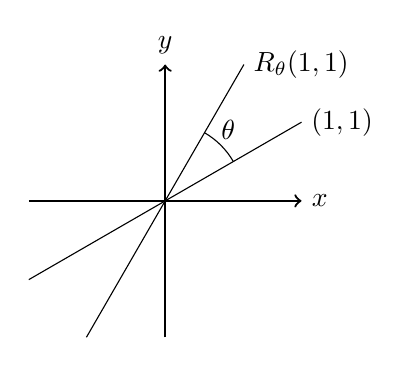
\begin{tikzpicture}
\draw[thick,->] (-1.732,0) -- (1.732,0)node[anchor=west] {$x$};
\draw[thick,->] (0,-1.732) -- (0,1.732)node[anchor=south] {$y$};
\draw (0.866,0.5) arc (30:60:1) ;
\draw[-] (-1.732,-1)--(1.732,1) node[right] {$\R (1,1)$};
\draw[-] (-1,-1.732)-- (1,1.732) node[right] {$\R R_\theta(1,1)$};
\node at (0.8,0.9){$\theta$};
\end{tikzpicture}
\end{Figure}
\end{center}

\end{Exemple}
\begin{Definition}[Image]

L'\defi{image} de $u$ est le sous espace vectoriel $u(E) = \{u(\Vect{x}):\Vect{x}\in  E\}$;
  on le note \defi{$\im u$}.\\
Par définition de la surjectivité, $\im u=E$ si et seulement $u$ est surjective. 
\end{Definition}
\begin{Definition}[Rang] Le \defi{rang} d'une  application linéaire $u$ est  la dimension de l'espace vectoriel $\Ima u$;
  on le note \defi{$\rg u$}.\\
\end{Definition}

\begin{Definition}[Noyau]
Le \defi{noyau} de $u$ est le le sous espace vectoriel $u^{-1}\{ \{\Vect{0_F}\}\} = \{x\in  E:u(\Vect{x}=\Vect{0_F}\}$;
on le note \defi{$\Ker u$}.
\end{Definition}

\begin{Proposition}[Caractérisation de l'injectivité par le noyau]  
$u$ est injective si et seulement si $\Ker u = \{\Vect{0_E}\}$.
\end{Proposition}

\begin{Demonstration}  
\begin{itemize}
\item Supposons que $u$ est injective.
 \begin{itemize}
\item $\Ker u \supset \{\Vect{0_E}\}$ : comme $\Ker u$ est un sous-espace vectoriel de $E$, il contient $\Vect{0_E}$
\item $\Ker u \subset \{\Vect{0_E}\}$ : soit $\Vect{x}\in \Ker u $. On a $u(\Vect{x})=\Vect{0_F}$. Comme $u$ est linéaire, $u(\Vect{0_E})=\Vect{0_F}$. Ainsi 
$u(\Vect{x})=u(\Vect{0_E})$. Comme $u$ est injective, $\Vect{x}=\Vect{0_E}$.
\end{itemize}
Du fait de la double inclusion $\Ker u = \{\Vect{0_E}\}$.
\item  Supposons que $\Ker u = \{\Vect{0_E}\}$.\\
soit $\Vect{x},\Vect{x'}\in E $ tel que $u(\Vect{x})=u(\Vect{x'})$. Alors $u(\Vect{x})-u(\Vect{x'})=\Vect{0_F}$ et par linéarité $u(\Vect{x}-\Vect{x'})=\Vect{0_F}$. Donc $\Vect{x}-\Vect{x'}\in \Ker u= \{\Vect{0_E}\}$. Ainsi $\Vect{x}-\Vect{x'}=\Vect{0_E}$. D'où $\Vect{x}=\Vect{x'}$.
\end{itemize}
\end{Demonstration}
\begin{Texte}
Pour démontrer une égalité entre deux ensembles, il faut prouver la double inclusion.    
En tant que sous-espace vectoriel de $E$, $\Ker u$ contient $\Vect{0}_E$, donc $\{\Vect{0}_E\}\subset \Ker u$. Ainsi démontrer que  $\Ker u = \{\Vect{0_E}\}$
et ainsi que $u$ est injective, il suffit en réalité de
montrer l'\impo{inclusion} : $\{\Vect{0_E}\}\subset \Ker u$.
\end{Texte}

\begin{Exemple}
Soit $\Fonction{u}{\R^3}{\R^2}{(x,y,z)}{(x+y+z,x-y)}$.\\
On a $u(x,y,z)=x(1,1)+y(1,-1)+z(0,1)$.
Donc $\Ima u$ est l'espace vectoriel engendré par la famille $((1,1),(1,-1),(0,1))$ d'où $\Ima u=\R^2$. Ainsi $u$ est surjective et $\rg u=2$.
$$(x,y,z)\in \Ker u \Leftrightarrow u(x,y,z)=(0,0)  \Leftrightarrow \begin{cases}x+y+z=&0\\x-y=&0\end{cases}\Leftrightarrow(x,y,z)=x(1,1,-2).$$
Donc $\Ker u =\R (1,1,2).$ Ainsi $u$ n'est pas injective.
\end{Exemple}
\begin{Exemple}[Dérivée polynomiale]
Soit $P=a_0+a_1 X+\dots + a_n X^n \in \R_n[X].$
On a $\Phi_3(P)=P'=a_1+a_2 .2X+\dots  + a_n.nX^{n-1}$.
Donc $\Ima \Phi_3$ est l'espace vectoriel engendré par la famille $(1,X,2X,\dots,nX^{n-1})$, soit $\Ima \Phi_3=\R_{n-1}[X].$ $\Phi_3$ n'est pas surjective $\rg u=\dim \R_{n-1}[X]=n $.
 $$P\in \Ker \Phi_3  \Leftrightarrow \Phi_3(P)=0  \Leftrightarrow P'=0\Leftrightarrow \exists a\in \R : P=a.$$
Donc $\Ker \Phi_3 =\R_{0}[X].$ $\Phi_3$ n'est pas injective.
\end{Exemple}




\begin{Proposition}[Permutation de Vect et de l'image]
Soit $(\Vect{x_i})_{i\leq i \leq n }$ une famille de $E$ .\\
Alors $$ u(\text{Vect}((\Vect{x_i})_{i\leq i \leq n}))=\text{Vect}\left(u(\Vect{x_i})\right)_{i\leq i \leq n}.$$
\end{Proposition}
\begin{Demonstration}
\begin{itemize}
\item  $u(\text{Vect}((\Vect{x_i})_{i\leq i \leq n}))\subset\text{Vect}\left(u(\Vect{x_i})\right)_{i\leq i \leq n}$:\\
Soit $\sum_{i=1}^n \lambda_i \Vect{x_i}\in \text{Vect}((\Vect{x_i})_{i\leq i \leq n})$.\\
Comme $u(\sum_{i=1}^n \lambda_i \Vect{x_i})\overbrace{=}^{\text{linéarité}}\sum_{i=1}^n \lambda_i u( \Vect{x_i})$, $u(\sum_{i=1}^n \lambda_i \Vect{x_i})$ s'exprime comme combinaison linéaire des vecteurs $\left(u(\Vect{x_i})\right)_{i\leq i \leq n}$ donc appartient à $\text{Vect}\left(u(\Vect{x_i})\right)_{i\leq i \leq n}$
\item $u(\text{Vect}((\Vect{x_i})_{i\leq i \leq n}))\supset\text{Vect}\left(u(\Vect{x_i})\right)_{i\leq i \leq n}$: Raisonnement similaire.
\end{itemize}
Du fait de la double inclusion, on a bien $ u(\text{Vect}((\Vect{x_i})_{i\leq i \leq n}))=\text{Vect}\left(u(\Vect{x_i})\right)_{i\leq i \leq n}.$
\end{Demonstration}
\begin{Corollaire}[Image d'une base]
Soit $(\Vect{e_i})_{i\leq i \leq n}$ une base de $E$ .\\
Alors $$ \Ima u =\text{Vect}( \left(u(\Vect{x_i})\right)_{i\leq i \leq n})).$$
\end{Corollaire}
\begin{Demonstration}
Comme $ \Ima u =u(E)$ et $E=\text{Vect}(\Vect{e_i})_{i\leq i \leq n }$, d'après la proposition précédente, on obtient $ \Ima u =\text{Vect}( \left(u(\Vect{x_i})\right)_{i\leq i \leq n})).$
\end{Demonstration}

\begin{Proposition}[Linéarité de l'inverse]
Si $u$ est un isomorphisme, alors $u^{-1}$ est également linéaire.
\end{Proposition}
\begin{Demonstration}  
Soit $\Vect{x},\Vect{x'}\in F $ et $\lambda\in\K$.\\
On a $u(u^{-1}(\lambda\Vect{x}+\Vect{x'}))=\lambda\Vect{x}+\Vect{x'}$. De plus, $u(\lambda u^{-1}(\Vect{x})+ u^{-1}(\Vect{x'}))\overbrace{=}^{\text{linéarité}}\lambda u( u^{-1}(\Vect{x}))+ u(u^{-1}(\Vect{x'}))=\lambda\Vect{x}+\Vect{x'}.$. Ainsi $u(u^{-1}(\lambda\Vect{x}+\Vect{x'}))=u(\lambda u^{-1}(\Vect{x})+ u^{-1}(\Vect{x'}))$. Comme $u$ est injective,  $u^{-1}(\lambda\Vect{x}+\Vect{x'})=\lambda u^{-1}(\Vect{x})+ u^{-1}(\Vect{x'})$.\\
 $u^{-1}$ est donc linéaire.
\end{Demonstration}





\subsection{Effet d'une applications linéaire sur la dimension}
\begin{Texte}
Une application linéaire, $u:E\to F$ ne peut que réduire la dimension de son ensemble de définition. 
\begin{center}
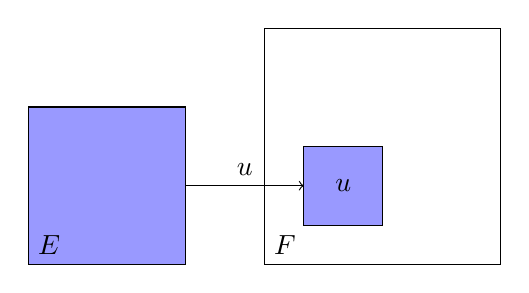
\begin{tikzpicture}
\fill[blue!40!white, draw=black] (0,0) rectangle (2,2);
\draw  (0,0) node[above right]{$E$};
\fill[white, draw=black] (3,0) rectangle (6,3);
\draw  (3,0) node[above right]{$F$};
\fill[blue!40!white, draw=black] (3.5,0.5) rectangle (4.5,1.5);
\draw  (4,1) node{$\im u$};
\draw[->]  (2,1) --node[above]{$u$} (3.5,1) ;
\end{tikzpicture}
\end{center}
L'application est injective si et seulement si: $\rg u =\dim E$.
\begin{center}
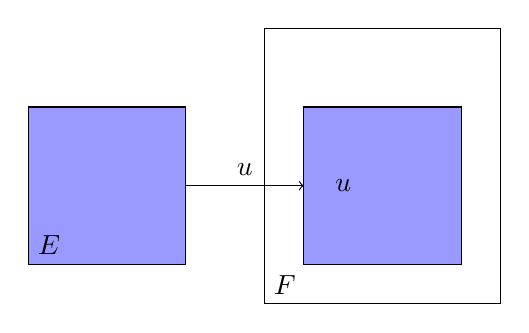
\begin{tikzpicture}
\fill[blue!40!white, draw=black] (0,0) rectangle (2,2);
\draw  (0,0) node[above right]{$E$};
\fill[white, draw=black] (3,-0.5) rectangle (6,3);
\draw  (3,-0.5) node[above right]{$F$};
\fill[blue!40!white, draw=black] (3.5,0) rectangle (5.5,2);
\draw  (4,1) node{$\im u$};
\draw[->]  (2,1) --node[above]{$u$} (3.5,1) ;
\end{tikzpicture}
\end{center}
L'application est surjective si et seulement si: $\rg u =\dim F$.
\begin{center}
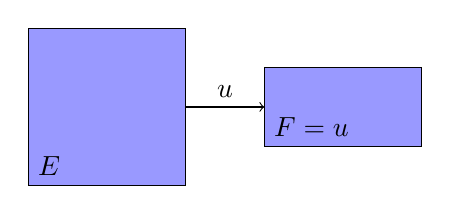
\begin{tikzpicture}
\fill[blue!40!white, draw=black] (0,0) rectangle (2,2);
\draw  (0,0) node[above right]{$E$};
\fill[blue!40!white, draw=black] (3,0.5) rectangle (5,1.5);
\draw  (3,0.5) node[above right]{$F=\im u$};
\draw[->]  (2,1) --node[above]{$u$} (3,1) ;
\end{tikzpicture}
\end{center}
L'application est un isomorphisme si et seulement si: $\rg u =\dim F=\dim E$.
\begin{center}
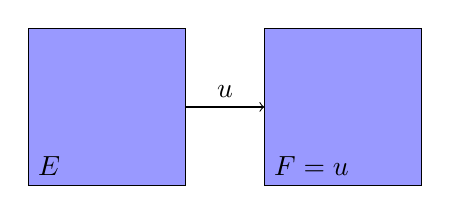
\begin{tikzpicture}
\fill[blue!40!white, draw=black] (0,0) rectangle (2,2);
\draw  (0,0) node[above right]{$E$};
\fill[blue!40!white, draw=black] (3,0) rectangle (5,2);
\draw  (3,0) node[above right]{$F=\im u$};
\draw[->]  (2,1) --node[above]{$u$} (3,1) ;
\end{tikzpicture}
\end{center}
\end{Texte}
\begin{Proposition}[Inégalité et égalité sur le rang]
Soit $u:E\to F$ une application linéaire.
\begin{itemize}
\item Si $F$ est de dimension finie, alors $\rg u \leq \dim F$, avec égalité si et seulement si $u$ est surjective.
\item  Si $E$ est de dimension finie, alors $\rg u \leq \dim E$, avec égalité si et seulement si $u$ est injective.
\end{itemize}
\end{Proposition}
\begin{Demonstration}
\begin{itemize}
\item 
Comme $\im u \subset F$, on a $\rg u =\dim  \im u\leq \dim F$. Pour l'égalité, on a  $u$ est surjective si et seulement si  $\im u =  F$ si et seulement si $\dim  \im u\leq \dim F$.
\item Soit $n$ la dimension de $E$ et $(\Vect{e_1},\dots,\Vect{e_n})$ une base de $E$. Comme $\im u=\operatorname{Vect}(u(\Vect{e_1}),\dots,u(\Vect{e_n}))$, $\dim  \im u\leq n$. Pour l'égalité, on a $\rg u \leq \dim E$ si et seulement si $u(\Vect{e_1}),\dots,u(\Vect{e_n})$ est une famille libre de $F$. 
\begin{itemize}
\item 
Supposons que $(u(\Vect{e_1}),\dots,u(\Vect{e_n}))$ est une famille libre de $F$. \\
Soit $\Vect{x}=\sum_{i=1}^n x_i\Vect{e_i} \in \Ker u$.
$$
\begin{aligned}
u(\vec{x})&=\Vect{0_F}&\\
u(\sum_{i=1}^n x_i\vec{e_i})&=\Vect{0_F}&\\
\sum_{i=1}^n x_i u(\vec{e_i})&=\Vect{0_F}&\text{ car u  linéaire}\\
\forall i\in \Intf{1}{n}:\quad x_i=0 &&\text{ car }  (u(\vec{e_1}),\dots,u(\vec{e_n})) \text{ libre}\\
\Vect{x}=\sum_{i=1}^n x_i\Vect{e_i}&=\Vect{0_E}&
\end{aligned}.
$$ Ainsi $\Ker u\subset \{\Vect{0_E}\}$. Donc $u$ est injective.
\item Supposons que $u$ est injective.\\
Soit $\lambda_1,\dots,\lambda_n\in\K$ tel que 
$$
\begin{aligned}
\sum_{i=1}^n\lambda_i u(\vec{e_i}))&=\Vect{0_F}&\\
u(\sum_{i=1}^n\lambda_i \vec{e_i}))&=\Vect{0_F}&\text{ car u  linéaire}\\
\sum_{i=1}^n\lambda_i \vec{e_i} &=\Vect{0_E}&\text{ car u  }\Ker u= \{\vec{0_E}\}\\
\forall i\in \Intf{1}{n}:\quad \lambda_i=0 &&\text{ car }  (\vec{e_1},\dots,\vec{e_n}) \text{ libre}\\
\end{aligned}.
$$
Donc $(u(\Vect{e_1}),\dots,u(\Vect{e_n}))$ est une famille libre de $F$.
\end{itemize}
\end{itemize}
\end{Demonstration}


\begin{Proposition}[Cas $\dim E = \dim F$]
Soit $u:E\to F$ une application linéaire tel que $\dim E = \dim F$.
\begin{center}
$u$ est un isomorphisme $\Leftrightarrow$ $u$ est injective $\Leftrightarrow$ $u$ est surjective.
\end{center}
Soit $u:E\to E$ une application linéaire tel que $\dim E$ est finie.
\begin{center}
\begin{tabular}{ccccc}
$u$ est un isomorphisme& $\Leftrightarrow$& $u$ est injective &$\Leftrightarrow$ &$u$ est surjective \\
$u\in \mathcal{GL}(E)$ &$\Leftrightarrow$ &  $u$ est inversible à gauche &$\Leftrightarrow$ &  $u$ est inversible à droite \\
$\exists v\in \LE: u\circ v =v \circ u = \mathrm{Id}_E$ &$\Leftrightarrow$ &  $\exists v\in \LE: v\circ u= \mathrm{Id}_E$  &$\Leftrightarrow$ &  $\exists v\in \LE: u\circ v= \mathrm{Id}_E$
\end{tabular}
\end{center}
\end{Proposition}

\begin{Demonstration}
\begin{itemize}
\item  Par hypothèse $\dim E = \dim F$. On a $u$ est injective si et seulement si : $\rg u = \dim E$ si et seulement si $\rg u = \dim F$   si et seulement si $u$ est surjective.
\item $u$ est inversible à gauche  si et seulement si  $\exists v\in \LE: v\circ u= \mathrm{Id}_E$   si et seulement si $u$ est injective si et seulement si $u$ est surjective  si et seulement si $\exists v\in \LE: u\circ v= \mathrm{Id}_E$ si et seulement si $u$ est inversible à droite.
\end{itemize}
\end{Demonstration}

\begin{Exemple}
Démontrer que l'application linéaire $\Fonction{u}{\R^2}{\R^2}{(x,y)}{ (x+y,x-y)}$ est un automorphisme.
\begin{Demonstration}
Comme $u$ est un endomorphisme, il suffit de démontrer qu'elle est injective.\\
$$(x,y)\in \Ker u \Leftrightarrow \begin{cases}x+y=0\\x-y=0\end{cases}  \Leftrightarrow  \begin{cases}x=0\\y=0\end{cases} $$ 
Donc $\Ker u =\{(0,0)\}.$
\end{Demonstration}
\end{Exemple}
\begin{Exemple}
Démontrer que l'application linéaire $\Fonction{u}{\R_n[X]}{\R_n[X]}{P}{  P-P}$  est un automorphisme.
\begin{Demonstration}
Comme $u$ est un endomorphisme, il suffit de montrer qu'elle est injective.\\
$$P\in \Ker u \Leftrightarrow P-P'=0  \Leftrightarrow  P=P'$$ 
Donc $\Ker u =\{0\}$ car $\deg(P)=\deg(P')$ si et seulement $P=0$.
\end{Demonstration}
\end{Exemple}


\subsection{Théorème du rang : $\dim E = \Rang u + \dim \Ker u$}
%Les dimensions du noyau et l'image d'une application linéaire sont liées.\\
%Soit $A=\begin{pmatrix} 1 &  0 &1\\ 0 &1 &1\\ 0 &1&1\end{pmatrix}$. On a $C_3=C_1+C2$.\\
%\textit{Image}  : $\im(A)=\mathrm{Vect}(C_1,C_2,C_3)\overbrace{=}^{C_3=C_1+C2}\mathrm{Vect}(C_1,C_2).$ Comme les vecteur $C_1$ et $C_2$ sont linéairement indépendants, $\dim (\im(A))=2$.\\
%\textit{Noyau}  : $\begin{pmatrix}x\\y\\z \end{pmatrix}\in \Ker(A)\Leftrightarrow xC_1 + yC_2 + zC_3= 0\overbrace{\Leftrightarrow}^{C_3=C_1+C2} (x+z)C_1 + (y+z)C_2 = 0$ \\$ \overbrace{\Leftrightarrow}^{C_1,C_2\text{linéairement indépendants} }\begin{cases}x=-z\\y=-z\end{cases} \Leftrightarrow \Ker(A)= \mathrm{Vect} \begin{pmatrix}1\\1\\-1 \end{pmatrix}$. Donc $\dim (\Ker(A))=1$.\\
%On observe que $\dim \Ker A +\dim \im A =$taille de la matrice. 

\begin{Texte}
 le théorème du rang lie le rang d'une application linéaire et la dimension de son noyau.
\end{Texte}
\begin{Lemme}[Factorisation]
Soit $E$ et $F$ deux $\K $-espaces vectoriels  et $u:E\to F$ une application linéaire.
Si $S$ est un supplémentaire de $\Ker u$, \\
Alors $u$ induit un isomorphisme de $S$ sur $\Ima u$,
c'est à dire que l'application linéaire
\[ \Fonction{u\vert_S}{S}{\Ima u}{\vec{x}}{u(\vec{x})} \]
est un isomorphisme.
\end{Lemme}
\begin{Demonstration}
\begin{itemize}
\item Injective :  Soit $\Vect{x}\in\Ker u\vert_S$ donc $x\in\Ker u$ et  $x\in S$. Comme $\Ker u$ et  $S$ sont supplémentaires, $\Ker u \cap S =\{\Vect{0_E}\}$. D'où $\Vect{x}=\Vect{0_E}$ et $\Ker u\vert_S=\{\Vect{0_E}\}$. 
\item Surjective : Soit $\Vect{y}\in \im u$ ainsi il existe $\Vect{x}\in E$ tel que $u(\Vect{x})=\Vect{y}$.  Comme  $\Ker u$ et  $S$ sont supplémentaires, il existe $\Vect{k}\in\Ker u$  et $\Vect{s}\in S $ tel que $\Vect{x}=\Vect{k}+\Vect{s}$. On  a :
$$
\begin{aligned}
u(\vec{x})&=\vec{y}&\\
u(\vec{k}+\vec{s})&=\vec{y}&\\
u(\vec{k})+u(\vec{s})&=\vec{y}&\text{ car u  linéaire}\\
 u(\vec{s})&=\vec{y}&\text{ car } \Vect{k}\in\Ker u.\\
\end{aligned}
$$
Ainsi $\Vect{s}$ est un antécédent de $\Vect{y}$ par l'application $u\vert_S$. Donc $u\vert_S$ est surjective.
\end{itemize}
\end{Demonstration}

\begin{Theoreme}[Théorème du rang]
Soit $E$ et $F$ deux $\K $-espaces vectoriels  et $u:E\to F$ une application linéaire.
On suppose que $E$ est de dimension finie.
Alors $\Ima u$ est de dimension finie et
\[ \dim E = \Rang u + \dim \Ker u. \]
\end{Theoreme}

\begin{Demonstration}
Comme $E$ est de dimension finie, $\Ker u$ possède un supplémentaire $S$ dans $E$. D'après le lemme de factorisation, comme $u\vert_S$ 
est un isomorphisme,   $\dim S = \dim \im u$. Comme  $S$ et $\Ker u$ sont supplémentaires dans $E$, on a $\dim S+\dim \Ker u=\dim E$. Finalement, on a 
$\dim \im u+\dim \Ker u=\dim E$.
\end{Demonstration}
%TODO exercices http://uel.unisciel.fr/mathematiques/espacevect1/espacevect1_ch04/co/apprendre_ch4_07_07.html et redémontrer effet d'une application linéaire 





\section{Application au système d'équations linéaires}
\begin{Theoreme}[Solutions d'une équation linéaire $u (\vec{x}) = \vec{y_0}$]
Soit $E$ et $F$ deux $\K $-espaces vectoriels, $u:E\to F$ une application linéaire et $\vec{y_0}\in F$.\\
L'ensemble des solutions de l'équation $u (\vec{x}) = \vec{y_0}$ est
\begin{itemize}
\item \propri{vide} si $\vec{y_0}\notin \im u$,
\item \propri{un espace affine} si $\vec{y_0}\in \im u$, c'est à dire de la forme $$\overbrace{\vec{x_0}}^{\text{Solution particulière}}+\overbrace{\Ker u}^{\text{Solutions homogènes}}=\{\vec{x_0}+\vec{x}:\vec{x}\in\Ker u\}.$$ 
\end{itemize}
\end{Theoreme}
\begin{Demonstration}
\begin{itemize}
\item Soit $y\notin \im u$. Il n'existe donc pas d'antécédent à la fonction $u$. Donc l'ensemble des solutions est vide.
\item Soit $y\in \im u$. Il existe au moins un antécédent à la fonction $u$ que l'on $\vec{x_0}$.\\
$\vec{x}$ est solution $ \Leftrightarrow u (\vec{x}) = \vec{y_0} \Leftrightarrow u (\vec{x}) = u (\vec{x_0}) \overbrace{\Leftrightarrow}^{\text{linéaire}} u(\vec{x}-\vec{x_0})=\Vect{0_F} \Leftrightarrow  \vec{x} - \vec{x_0} \in \Ker u  \Leftrightarrow \vec{x} \in \vec{x_0} +\Ker u.$
\end{itemize}
\end{Demonstration}
\begin{Exemple}[Taille d'un père et d'un fils]
Déterminer la structure des solutions de 
$$
\begin{cases}
{\color{red}x}+{\color{green}y}&={\color{blue}2,5}\\
{\color{red}-x}+{\color{green}y}&={\color{blue}0,5}
\end{cases}.
$$
\begin{Demonstration}
On pose $ \Fonction{u}{\R^2}{\R^2}{( {\color{red}x }   ,  {\color{green}y})}{ ({\color{red}x }   +  {\color{green}y},-{\color{red}x }   +  {\color{green}y})}$.
On cherche ainsi les solutions de l'équation :  $u( {\color{red}x }   ,  {\color{green}y})	 = ( {\color{blue}2,5}   {\color{blue}0,5})$.\\
$u$ est un endomorphisme. Comme $\Ker u=\{(0,0)\}$ car 
$
\begin{cases}
{\color{red}x}+{\color{green}y}&=0\\
{\color{red}-x}+{\color{green}y}&=0
\end{cases}\Leftrightarrow\begin{cases}
{\color{red}x}&=0\\
{\color{green}y}&=0
\end{cases}
$, $u$ est injective donc bijective.\\
 Comme $\im u=\R^2$, il existe une solution et comme $\Ker u=\{(0,0)\}$, cette solution est unique. 
\end{Demonstration}


\end{Exemple}




\end{document}
